\documentclass{article}

% Language setting
% Replace `english' with e.g. `spanish' to change the document language
\usepackage[english]{babel}

% Set page size and margins
% Replace `letterpaper' with `a4paper' for UK/EU standard size
\usepackage[letterpaper,top=2cm,bottom=2cm,left=3cm,right=3cm,marginparwidth=1.75cm]{geometry}

% Useful packages
\usepackage{amsmath}
\usepackage{graphicx}
\usepackage[colorlinks=true, allcolors=blue]{hyperref}
\usepackage{xcolor}
\usepackage{datetime}
\usepackage[section]{placeins} 
\usepackage{pdfpages}
\usepackage{float}

\title{ME136 Lab 3}
\author{Nathan Yacovetta, Aarchan Saxena, Jobanpreet Mutti, Radhika Marolia}
\date{October 19, 2023}

\begin{document}
\maketitle

\section{Contributions}

\begin{itemize}
\item Nathan Yacovetta: Worked on the write-up on Latex and helped with the code in the lab.
\item Aarchan Saxena: Performed lab tasks and collected all the data.
\item Jobanpreet Mutti: Used lab data to create all the plots necessary in the deliverables and helped with lab code.
\item Radhika Marolia: Worked on the write-up on Latex and questions/comments in the deliverables.
\end{itemize}

\section{Experimental Set-up:}

\subsection{Description}

\begin{itemize}
\item To begin setup, we included print statements to verify our axes and scale of the IMU. We confirmed the accelerometer axes followed our understanding by grabbing and maneuvering the orientation of the vehicle and checking direction of the movement, positive or negative. 

\item To calibrate the rate gyroscope's bias, we ran our code while the UAV was off and rested stationary on the flat and level ground. We then subtracted the measurement we received to calibrate the rate gyroscope as it should be zero while stationary.

\item Once we added the gyroscope estimator, we ran the code while the UAV was resting stationary flat on the ground again to see that the estimate began to deviate from zero. We then grabbed the vehicle and maneuvered it to have an upright orientation. We also rotate it through a half rotation to check the changes in pitch angle estimates as shown in Section 3.

\item We then added the accelerometer measurements and checked how it affected the estimator. We turned on the stationary vehicle to see how it initially affects the estimate. We also ran the code with different initial nonzero angles and grabbed the vehicle and performed a variety of rotations including full rotations of the vehicle about each axis.
\end{itemize}

\subsection{Screenshots}

\begin{figure} [H]
\centering
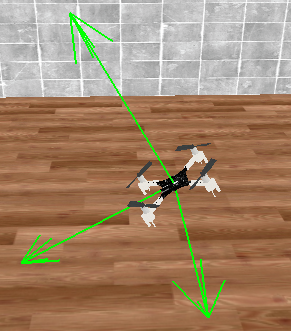
\includegraphics[scale=.75]{Lab3Setup.PNG}
\caption{Experimental Set up for Deliverable 3.2
\label{fig1}}
\end{figure}
\FloatBarrier
\vspace{24pt}

\section{For the 1D, purely integrating estimator, for 5 runs, record 30 seconds worth of data, for the vehicle initially turned off:}

\subsection {Part A}
The plots of our pitch angle estimates and y rate gyroscope data are shown below:

\begin{figure} [H]
\centering
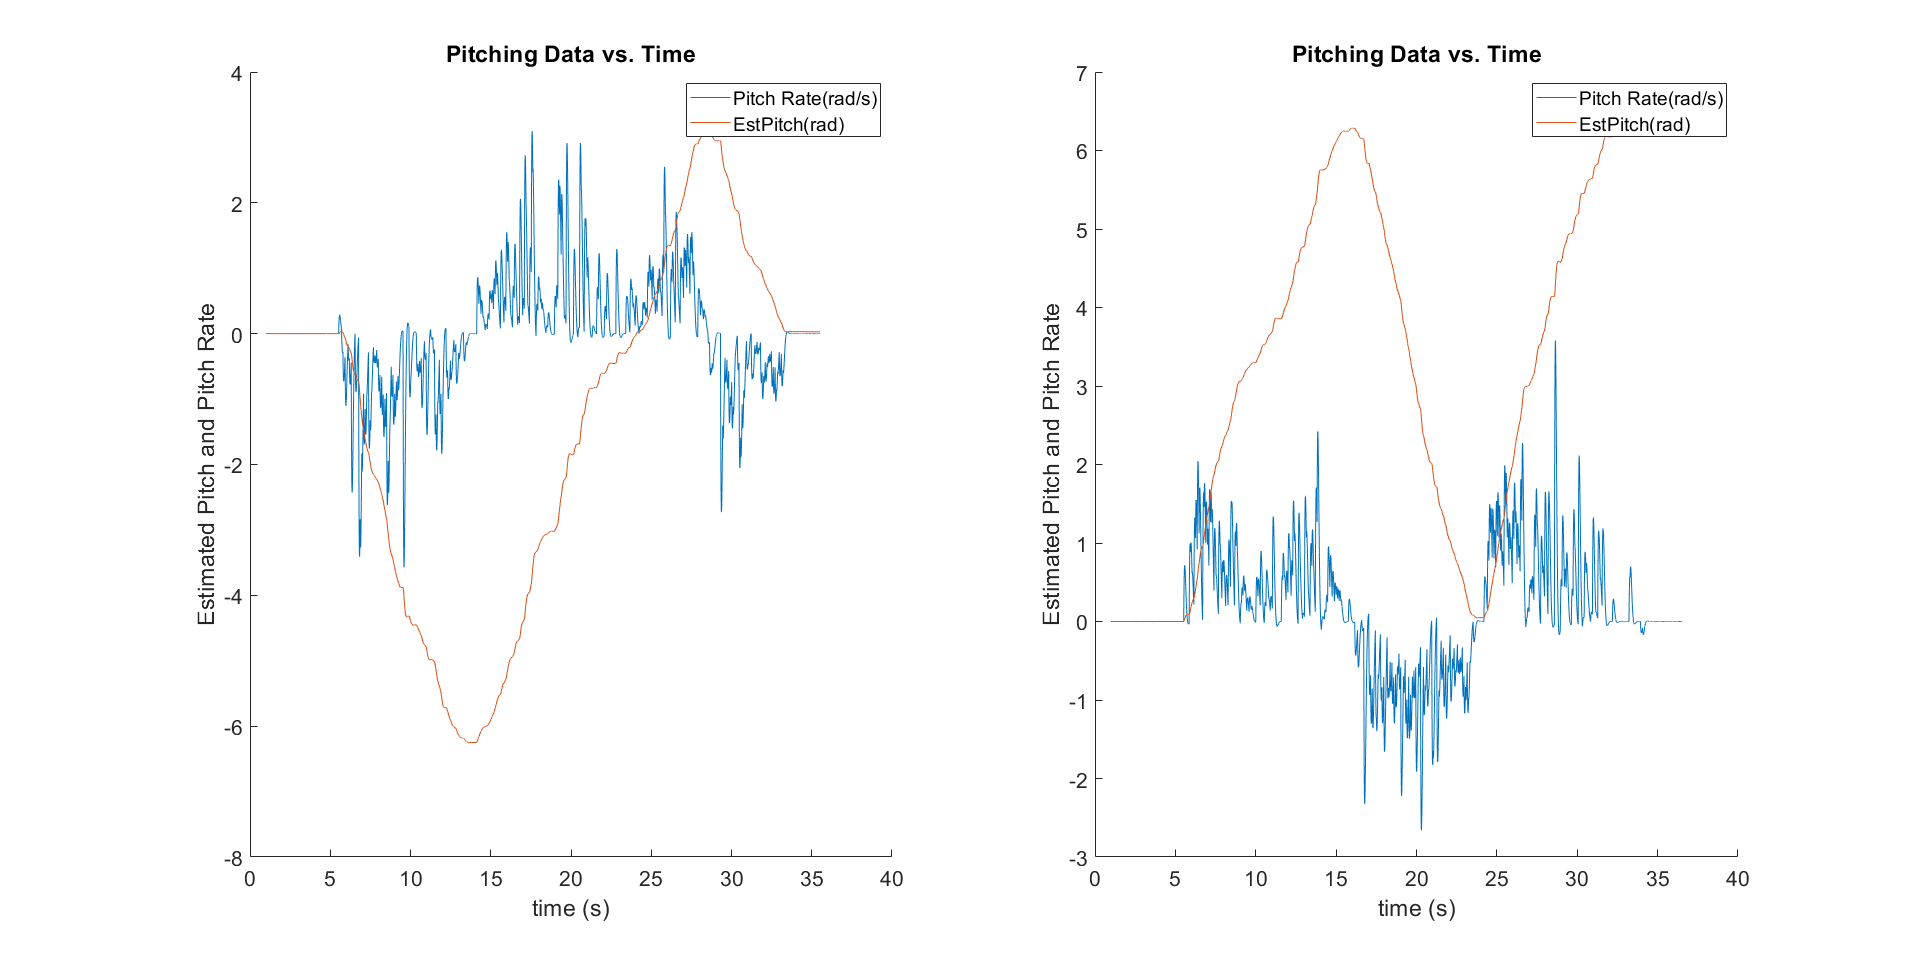
\includegraphics[scale=.25]{ME136Lab 3Q3aPic1.png}
\caption{Pitch Data VS Time: Runs 1 and 2 \label{fig2}}
\end{figure}
\FloatBarrier
\vspace{24pt}

\begin{figure} [H]
\centering
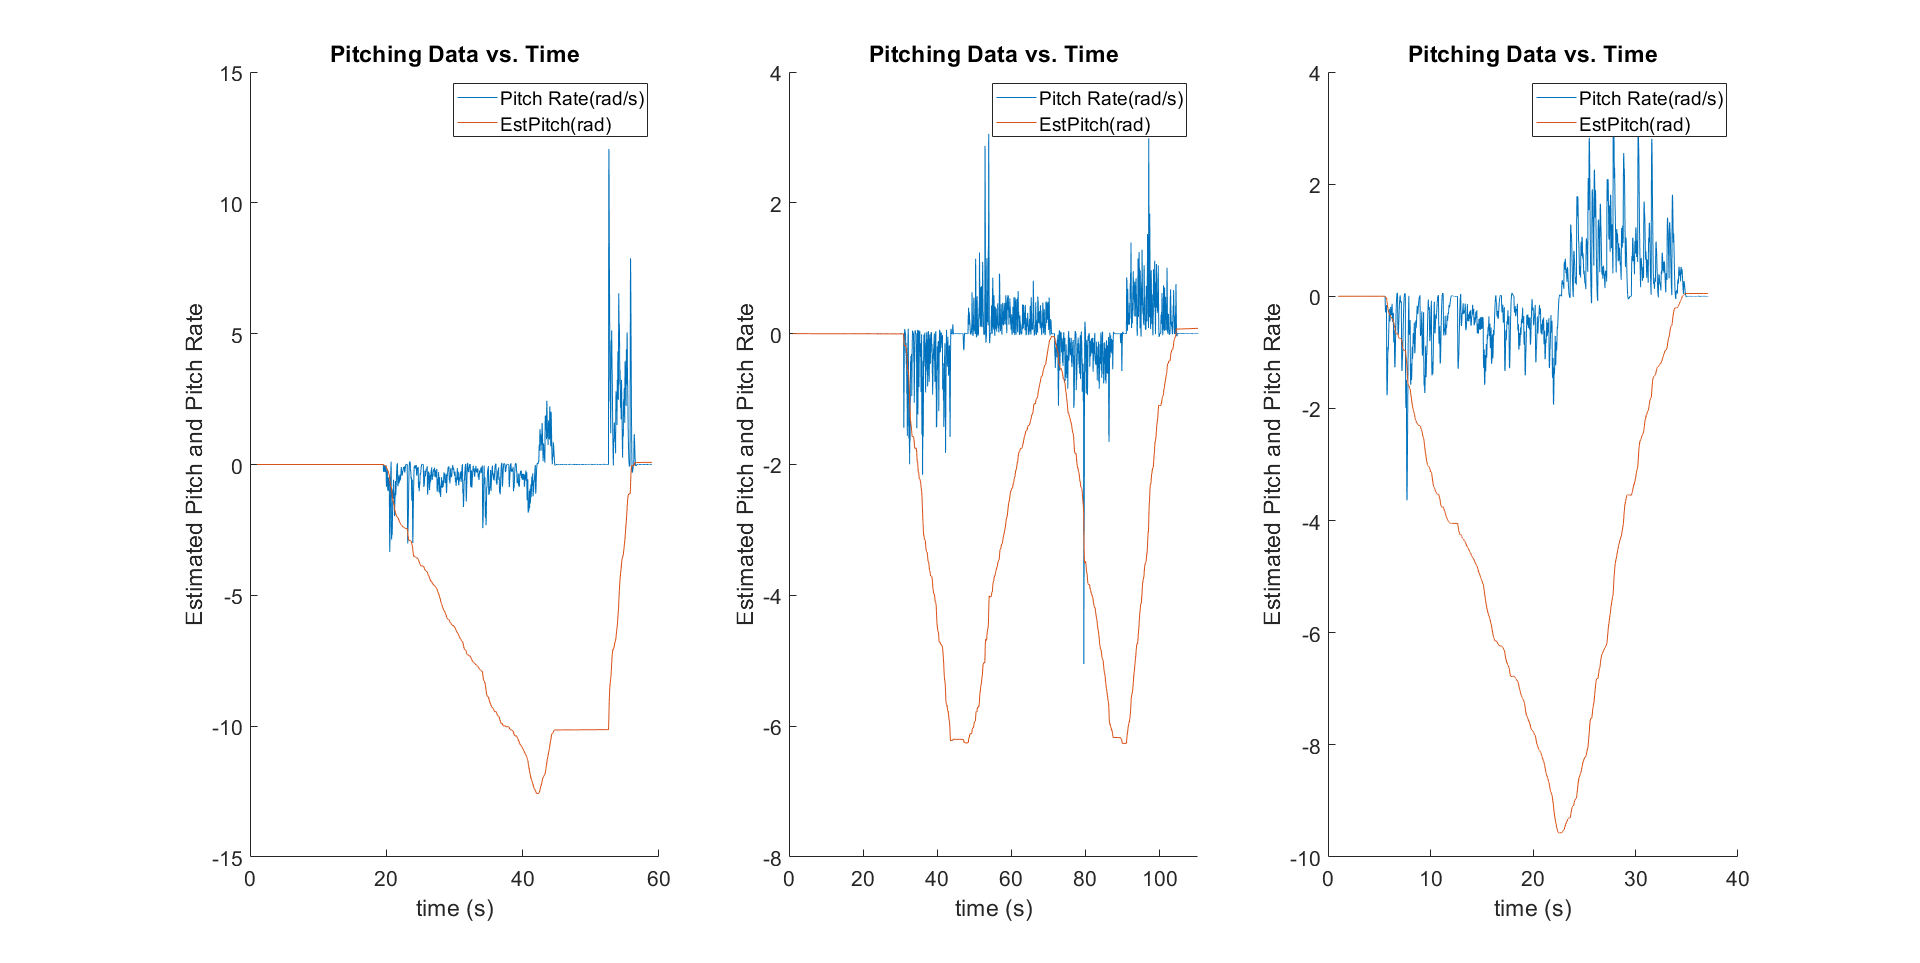
\includegraphics[scale=.30]{ME136Lab 3Q3aPic2.png}
\caption{Pitch Data VS Time: Runs 3, 4, and 5 \label{fig3}}
\end{figure}
\FloatBarrier
\vspace{24pt}

We used the raw data in our plots because we did not observe much of a difference between the raw data and corrected data.

\subsection {Part B}

A "excessive" attitude depends heavily on the vehicle and the purpose of its mission. A consumer drone may have over 10 degrees of offset while still maintaining functionality while a weather satellite would be nonfunctional with more than a few arcseconds of offset. For a generalized assumption, we assume over 1 degree of offset to be excessive. This allows for higher precision tasks to still be performed without being overconstrained by extreme precision tasks that would be unsuitable for the small drone used in our simulations. In our testing, it took an average of 5 minutes before our estimated pitch reached 1 degree while sitting at standstill.

\section{For the 1D estimator that incorporates the accelerometer:}

\subsection{Part A}
We analyzed the value of $\rho$ via a binary search method. Multiple $\rho$ values were used and each rotated the UAV by 30 degrees to identify how the estimated pitch changed. After isolating values of $\rho = 0.005$ which was too low and $\rho = 0.05$ which was too high, $\rho = 0.01$ was tested and identified as the ideal value for our simulations. Using $\rho = 0.05$ led to the output of the expected pitch being too much like a step function, with it changing much more based on the measured value from the accelerometer. In contrast, with $\rho = 0.005$, the measured value from the accelerometer is used much less, which can lead to a large run-away in the estimated pitch as it will be mainly reliant on the integrator.
\begin{figure} [H]
\centering
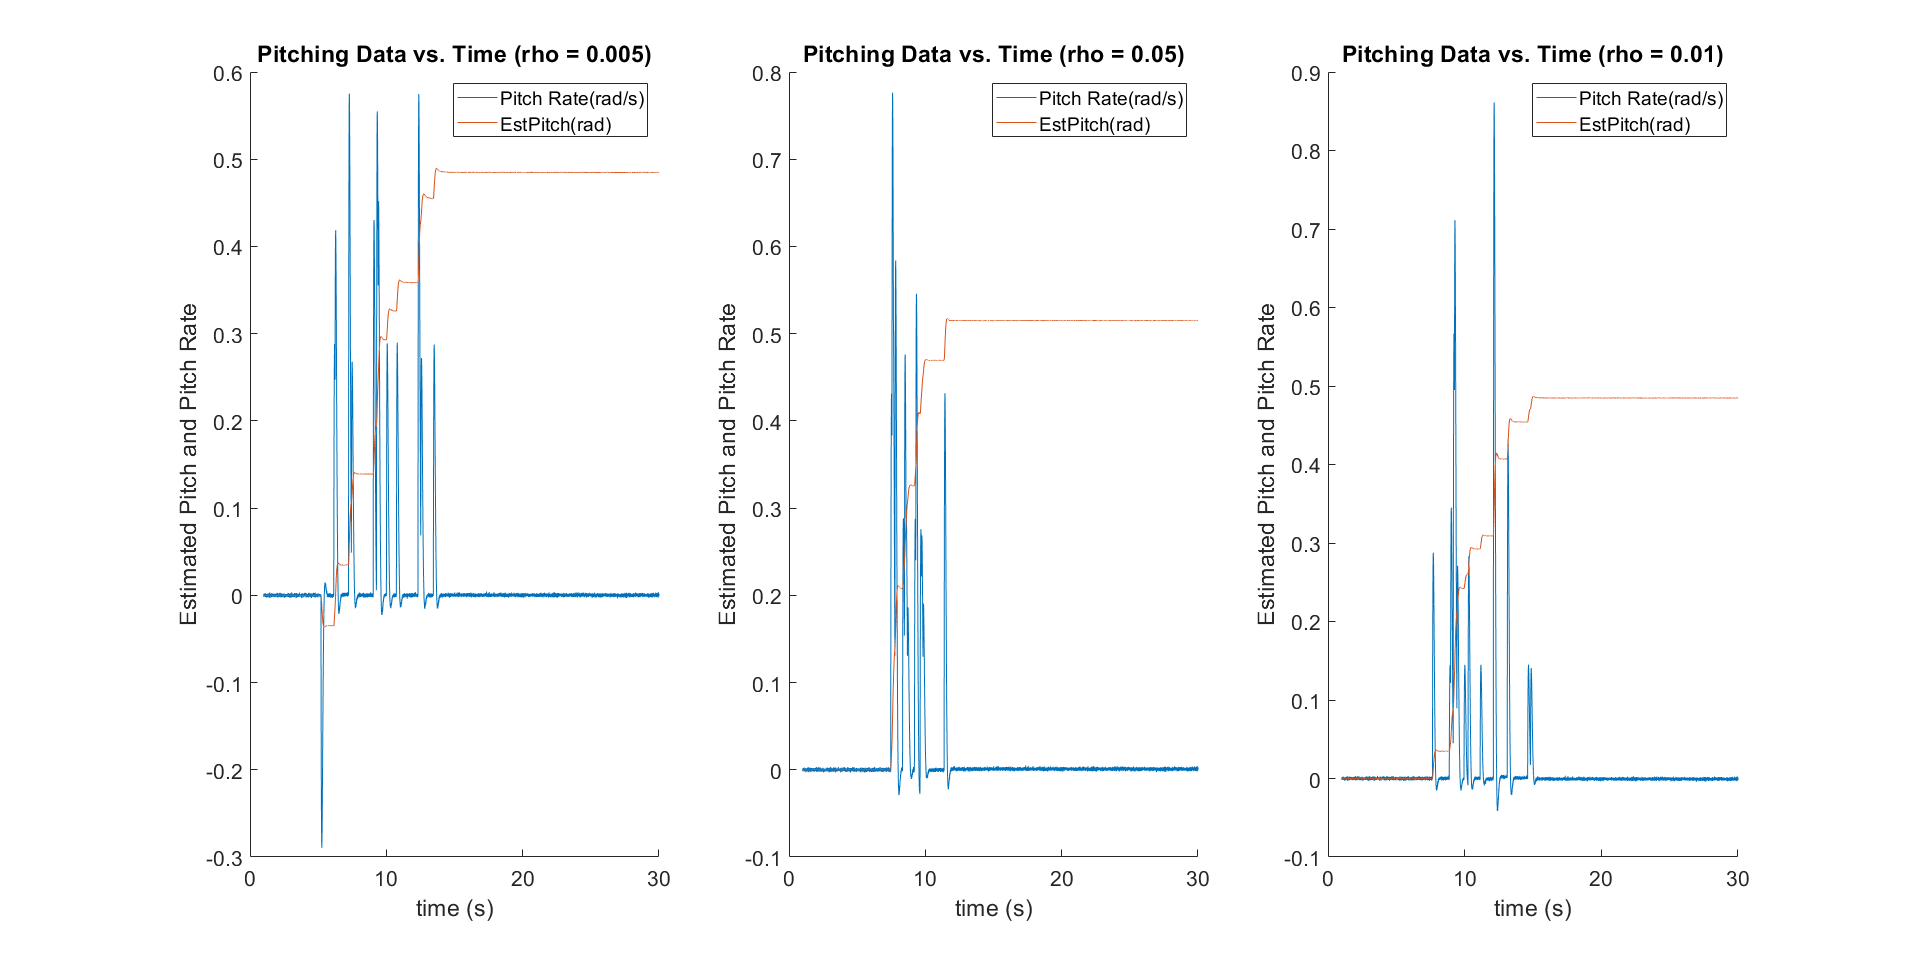
\includegraphics[scale=.25]{extracreditnew.png}
\caption{Pitch Data VS Time: Runs 1,2, and 3 \label{fig4}}
\end{figure}
\FloatBarrier
\vspace{24pt}

\subsection{Part B}
Plots of our attitude estimate and rate gyroscope data are shown below:

\begin{figure} [H]
\centering
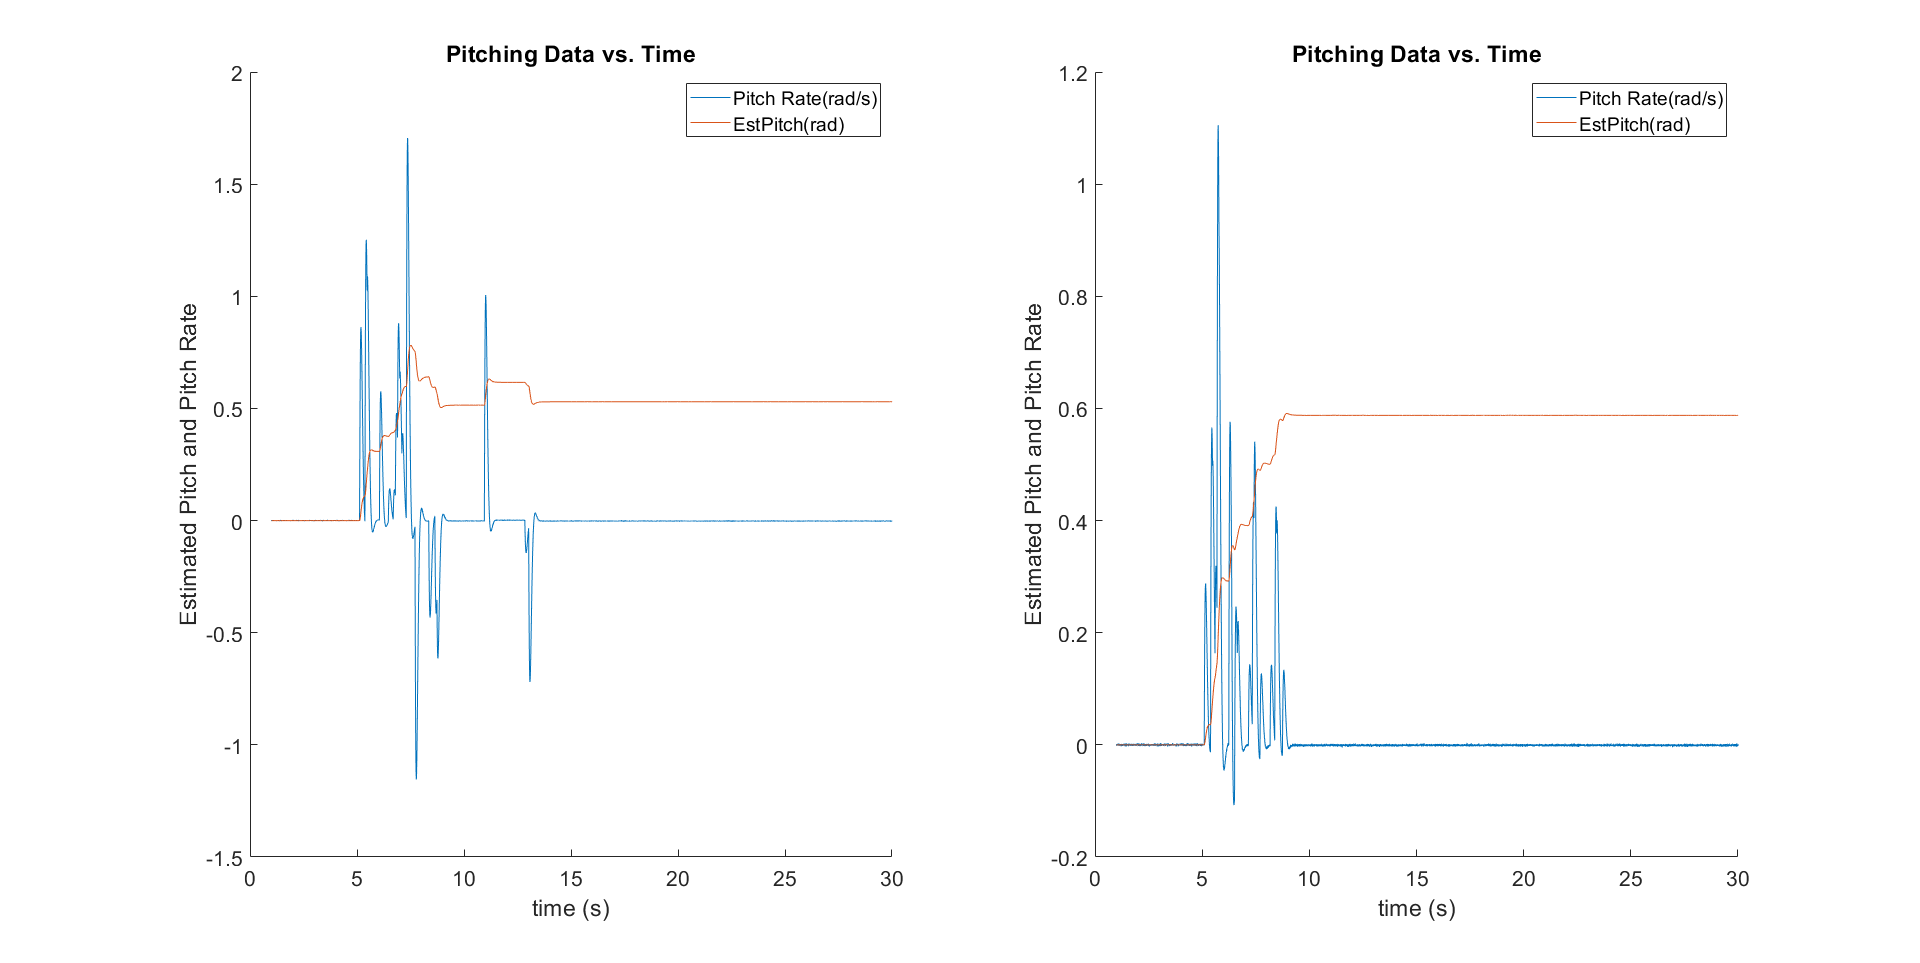
\includegraphics[scale=.25]{FD42.png}
\caption{Pitch Data VS Time: Runs 1 and 2 \label{fig4}}
\end{figure}
\FloatBarrier
\vspace{24pt}

\begin{figure} [H]
\centering
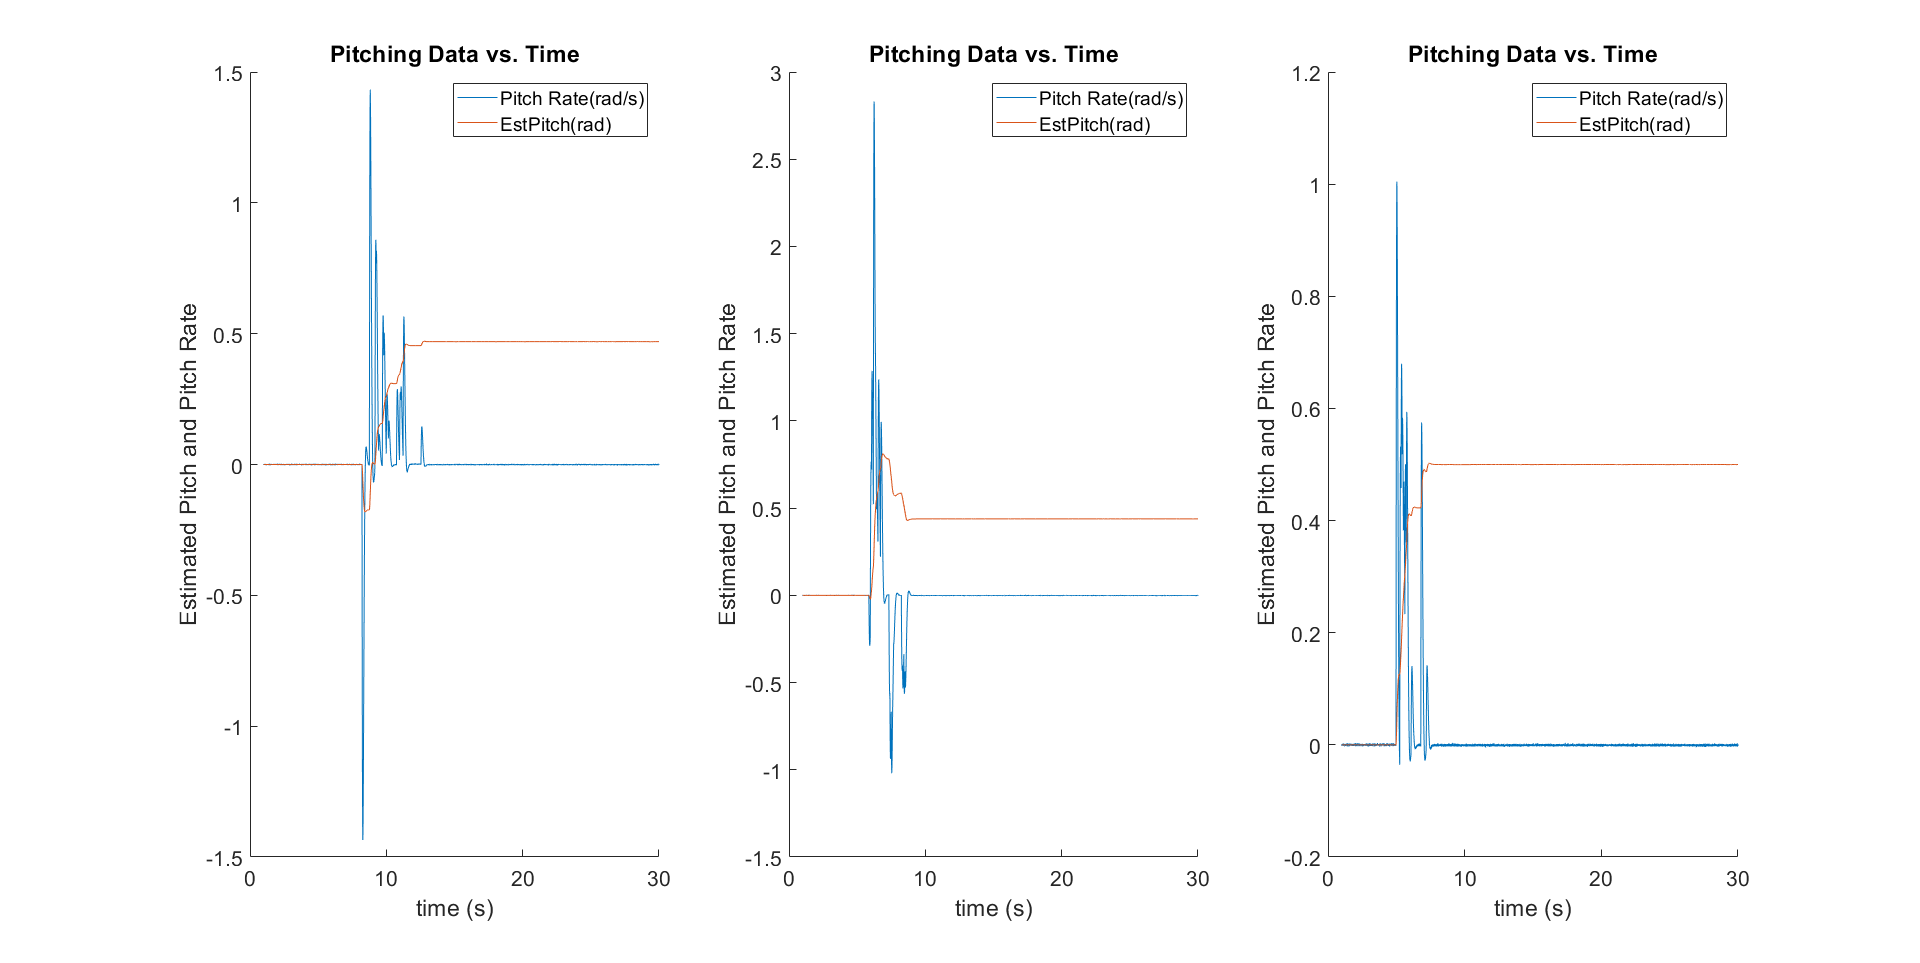
\includegraphics[scale=.30]{FD4.png}
\caption{Pitch Data VS Time: Runs 3, 4, and 5 \label{fig5}}
\end{figure}
\FloatBarrier
\vspace{24pt}

From these plots, we see that the estimator's output is relatively accurate. The upward and downward trends of the estimator output follow the increases and decreases in the pitch rate measured by the rate gyroscope. The estimator output remains zero and stays steady while the UAV remains stationary in the first five seconds of each run.

\section{For the 3D Estimator:}

\subsection{Estimation Error}
From our data and tables, we see that the estimation error is very minimal from the repeated turning tests. After multiple sets of movement, the pitch is able to return to a near zero radian value. However the estimation error still occurs because of the looping cycle of the estimator. The system estimates by combining the data from the current cycle of the main loop in our code with the data from the past loop to identify the difference. However, this value is only gathered at discrete time intervals and is averaged out. By gathering data at more frequent intervals in our main loop, we would be able to smooth out the error buildup by more accurately recording the UAV's motion.

\subsection{Representative Run Plot}
A plot of a representative run with the 3D estimator that shows all three angles is shown below. The motion ends where the pitch rate drops to zero and remains steady.

\begin{figure} [H]
\centering
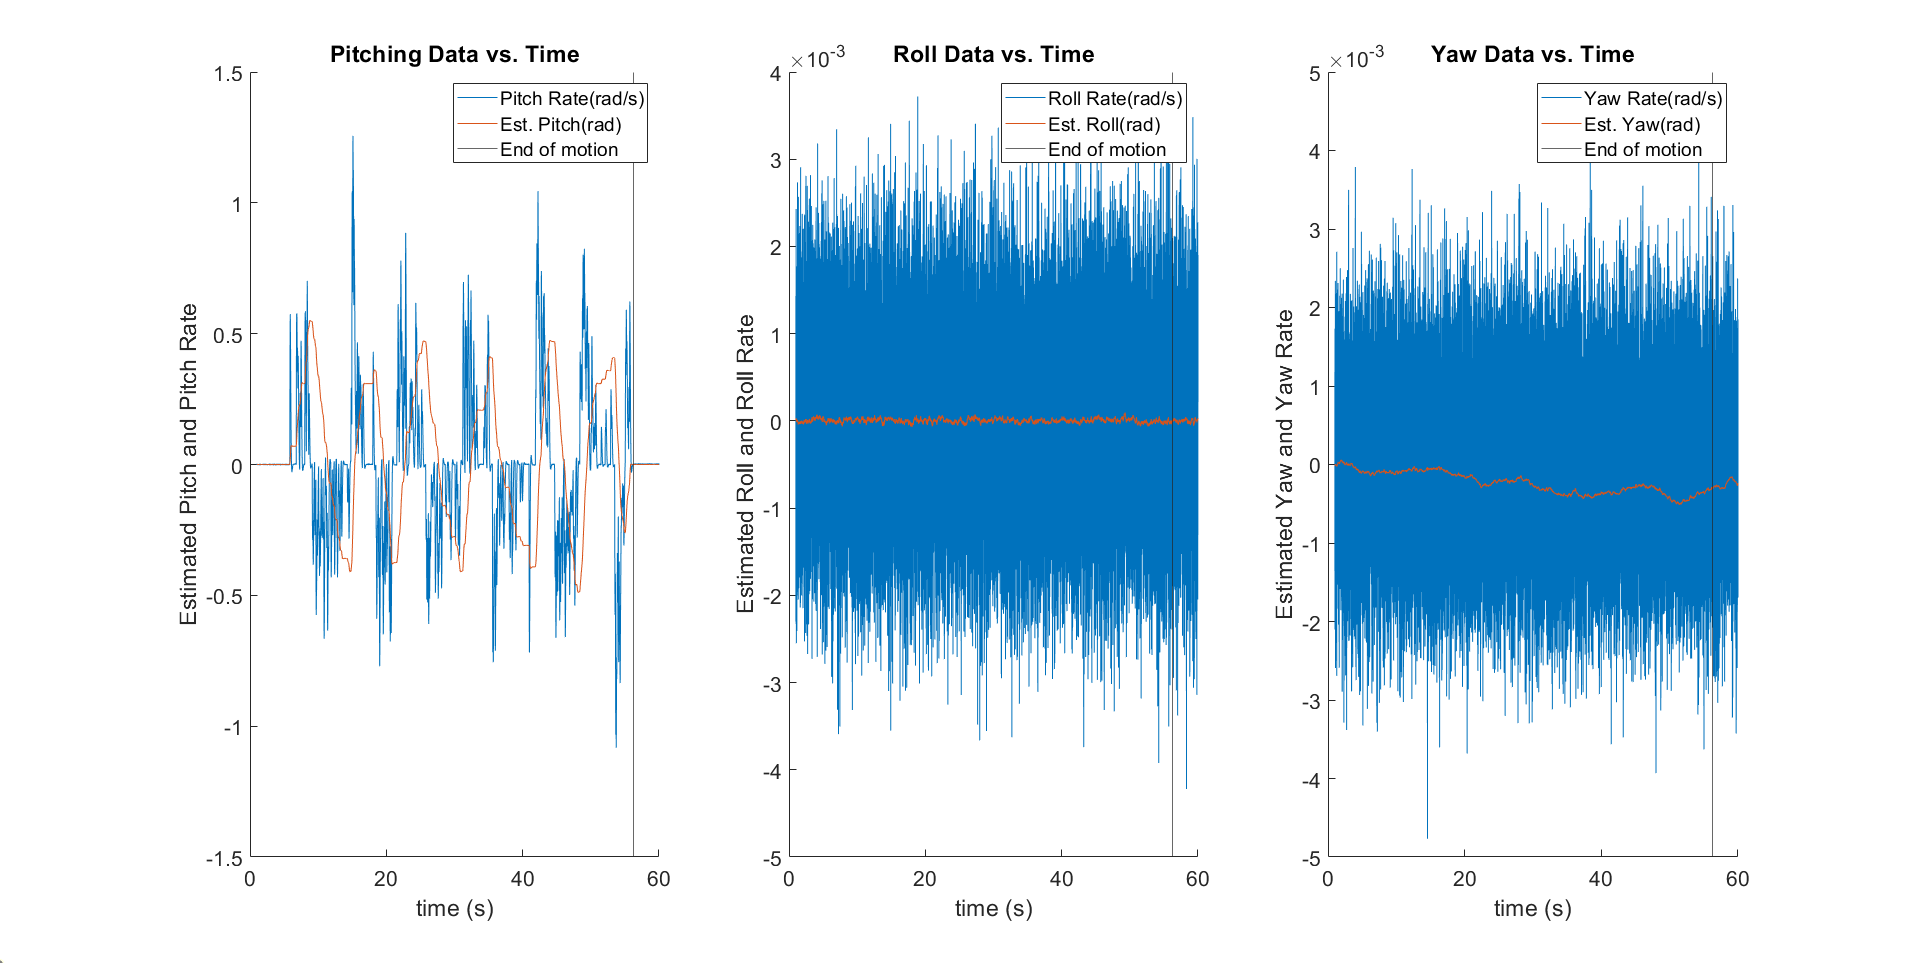
\includegraphics[scale=.30]{deliverable 5 3 graphs.png}
\caption{Pitch, Roll, and Yaw Data VS Time: 3D Estimator \label{fig6}}
\end{figure}
\FloatBarrier
\vspace{24pt}

\section{MainLoop Function}

\subsection{Virtual Machine Code}

On the page below is the full listing of our UserCode with comments where we added code to the MainLoop function for lab 3 starting at line 45:
\includepdf[pages=-]{Lab3Usercode.pdf}

On the page below is the full listing of our UtilityCode with comments:
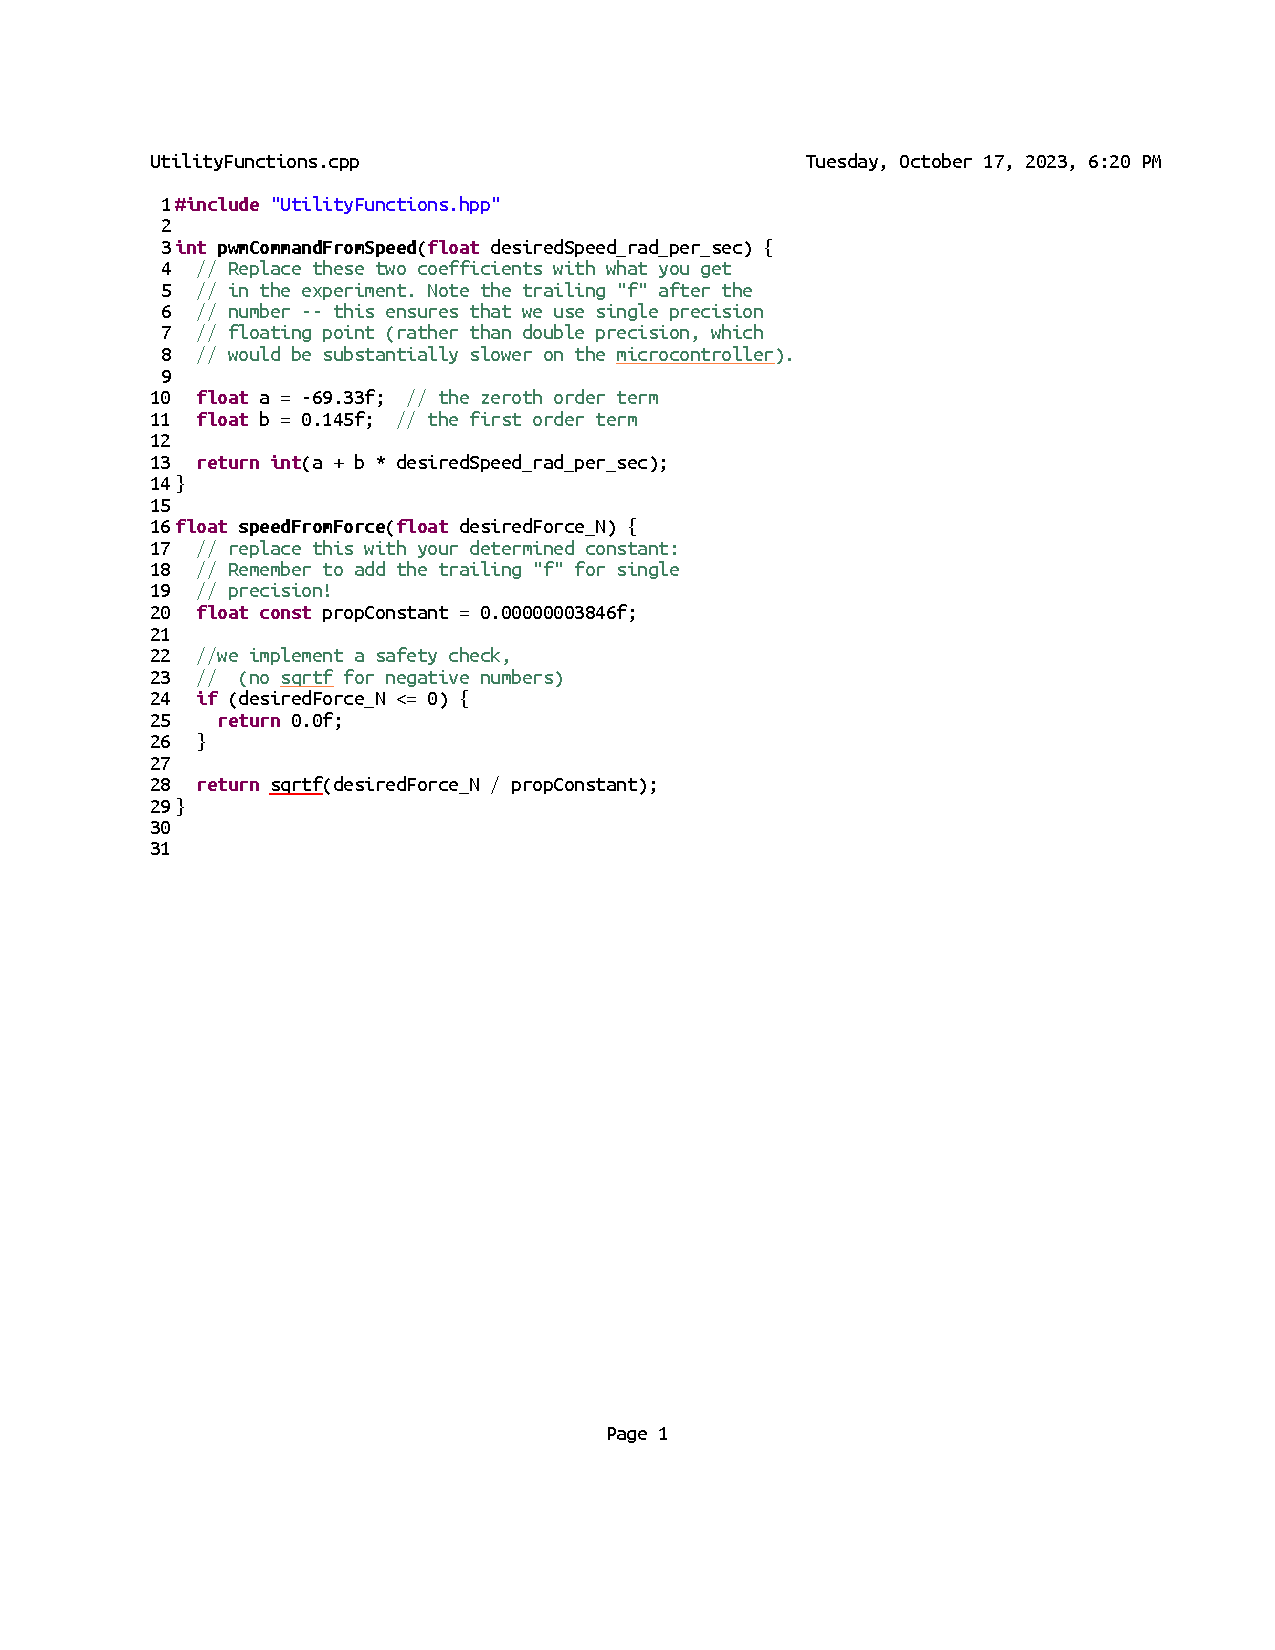
\includepdf[pages=-]{Lab3UtilityCode.pdf}

\subsection{Matlab Code} %if you guys wanna add this at the end
On the page below is our Matlab code we used to plot the pitch data versus time for each of our sections.

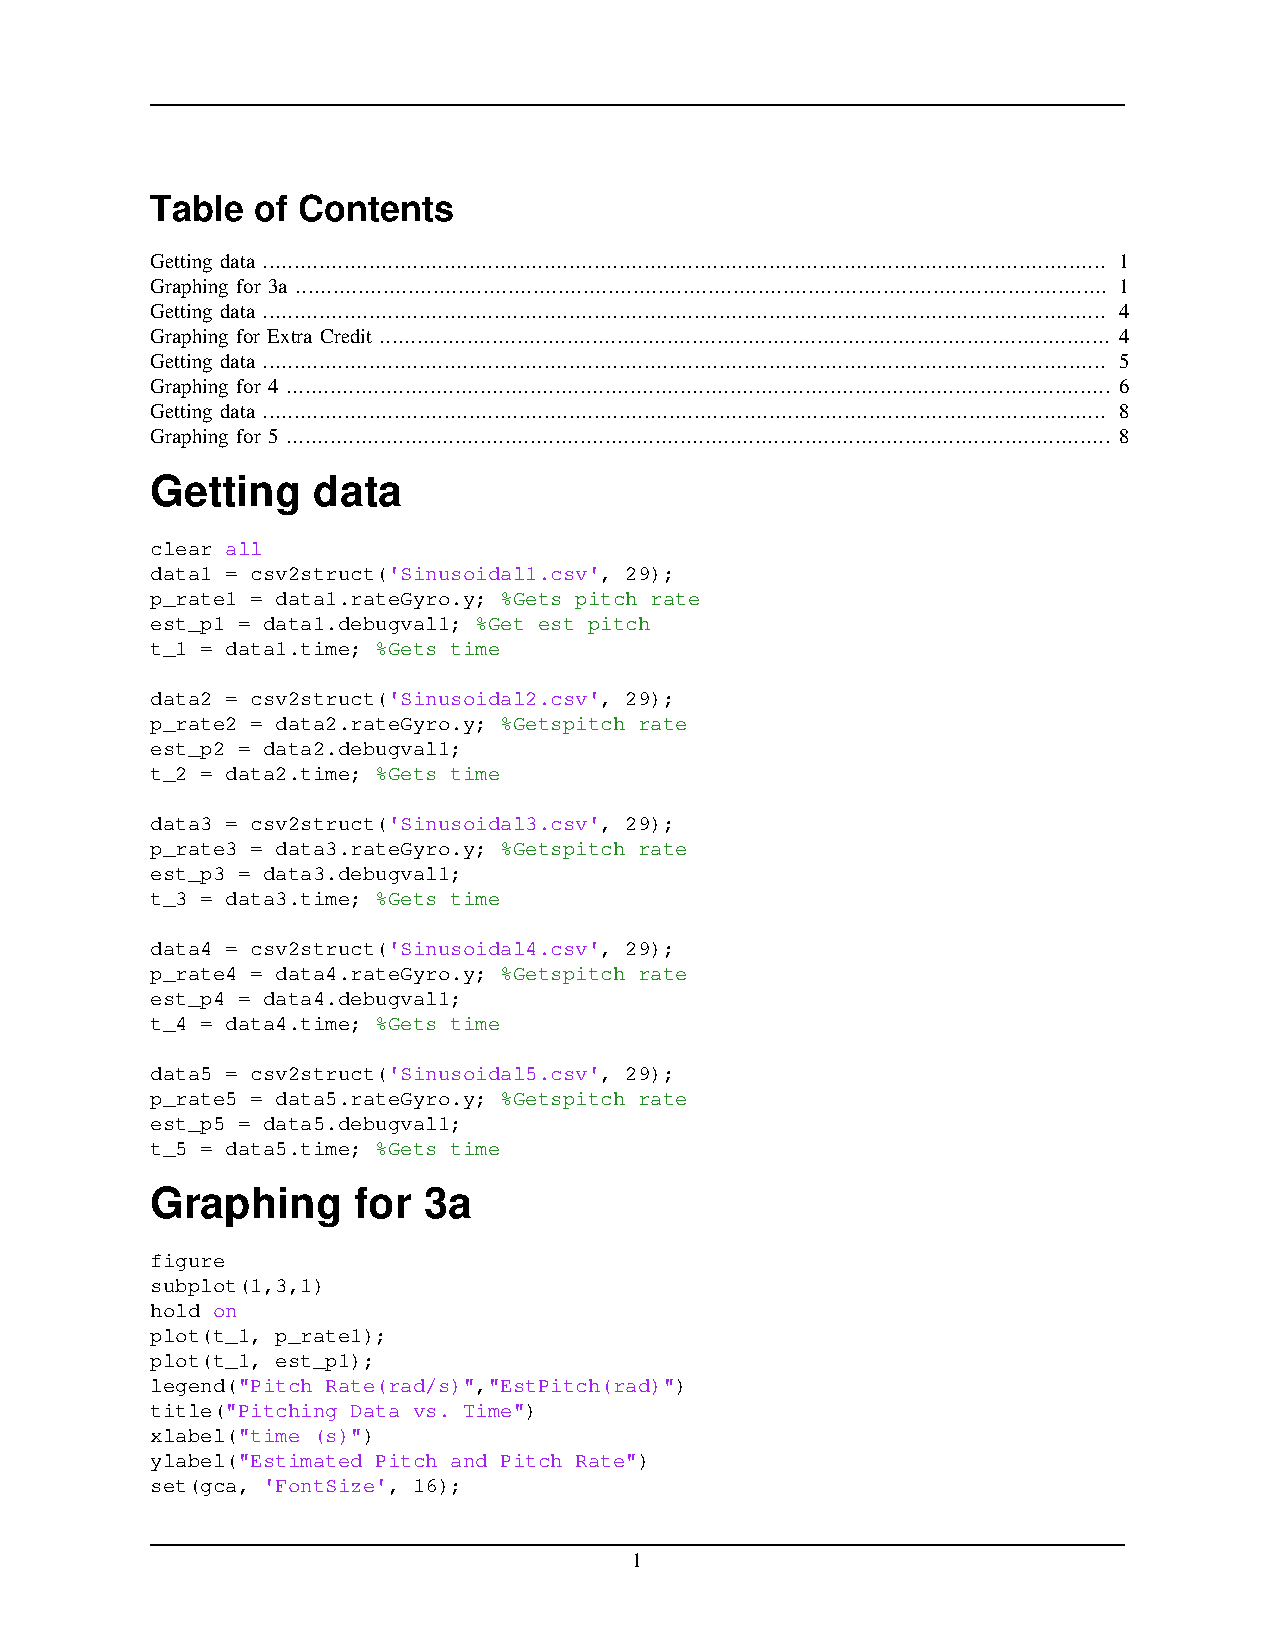
\includepdf[pages=-]{Lab3.pdf} %just change this

\end{document}
